\section{Experiments}
\label{sec:experiments}

\paragraph{Setup.}
Train has 9{,}392 labelled images (32{,}533 boxes); val (1{,}426) and test (2{,}065) are scored by the course
leaderboard against the reference (val 93.31 / 26.13, test 93.99 / 25.41 macro-F1 / mAP).
Local numbers are ND $\Delta_m$ (\cref{eq:dm}) with our decoding, mean\,$\pm$\,std over seeds 0--2 where three are
given.
We use PyTorch 2.9 (bf16), Ultralytics 8.4.189 for YOLO26's network, loss and assigner, torchvision NMS and the
course's data and metric code; our code adds the multi-task model, training loop, augmentations, decoding, SWA and the
holdout tools.
Training: AdamW~\cite{loshchilov2019adamw} (lr and weight decay $5{\times}10^{-4}$), 3 warm-up epochs, cosine to
1\,\%, gradient clip 10, EMA 0.9998, batch 16, 350 epochs.
\textbf{Compute:} three NVIDIA L40S (46\,GB), up to four of our runs per GPU.
The final model trained in 8.96\,h (wall clock, its GPU shared with one other run) plus 0.24\,h of SWA, peaking at
7.0\,GB; inference takes 2.45\,ms per image at batch 16 and 21.5\,ms at batch 1 (forward and decoding, 1.2\,GB).
The whole project, five designs and the baseline runs included, occupied about 400 GPU-hours (union of busy intervals
per GPU; the runs' own clocks sum to 591\,h).
Pretrained weights, none trained on SAR data: the final model uses only YOLO26-L's COCO weights (Ultralytics' v8.4.0
release); we also tried YOLO26-X and RT-DETR-L (same release) and ConvNeXt-B~\cite{liu2022convnext} (timm
\nolinkurl{convnext_base.fb_in22k_ft_in1k}), and earlier designs used ViT-B/16 (timm
\nolinkurl{vit_base_patch16_224.augreg_in21k}), TerraMind-1.0-base~\cite{jakubik2025terramind} (IBM/ESA) and
torchvision's COCO Faster R-CNN R50-FPN v2.

\subsection{Main results}
\label{sec:main}

\begin{table}[t]
  \centering
  \footnotesize
  \setlength{\tabcolsep}{3.4pt}
  \begin{tabular}{@{}lcccccc@{}}
    \toprule
    & \multicolumn{2}{c}{Params (M)} & \multicolumn{2}{c}{Val} & \multicolumn{2}{c}{Test} \\
    \cmidrule(lr){2-3}\cmidrule(lr){4-5}\cmidrule(l){6-7}
    Model & train. & total & mAP & $\Delta_m$ & mAP & $\Delta_m$ \\
    \midrule
    ViT-B/16 + LoRA (ref.)        & 21.0 & 107 & 26.1 & 0.0   & 25.4 & 0.0 \\
    TerraMind + MoE-LoRA          & 21.1 & 106 & 28.8 & +4.4  & 27.8 & +3.8 \\
    ViT-B/16 full FT$^\dagger$    & 106  & 106 & 32.0 & +11.8 & 31.8 & +13.5 \\
    \midrule
    \textbf{Ours} (YOLO26-L MT)   & 26.2 & 26.2 & \textbf{49.9} & \textbf{+45.9} & \textbf{49.7} & \textbf{+48.7} \\
    \bottomrule
  \end{tabular}
  \caption{\textbf{Leaderboard results.} Baselines: the course's runs, mean of 3 seeds; $^\dagger$over budget. Ours: the
  posted single model (seed 6 + SWA), macro-F1 93.98 / 95.61; 8th of 9 teams on val, 6th of 8 on test (6 Nov).}
  \label{tab:main}
\end{table}

\Cref{tab:main} compares our posted model with the course baselines.
It raises val and test mAP from 28.8 and 27.8 to 49.9 and 49.7 with a quarter of the parameters, while macro-F1 stays at
the reference's level.
The gain is almost all detection, and so is the gap to the leading teams (val mAP up to 60.8).
Phase 2 tests the checkpoint of our posted val entry unchanged, as required.

\subsection{From adapted ViTs to a compact detector}
\label{sec:journey}

\begin{table}[t]
  \centering
  \footnotesize
  \setlength{\tabcolsep}{2.6pt}
  \begin{tabular}{@{}llcr@{}}
    \toprule
    Design & Key idea (pretraining) & Train.\,(M) & Val $\Delta_m$ \\
    \midrule
    DetailLoRA  & MoE-LoRA + detail branch (EO)     & 21.5 & +4.6 \\
    WideLoRA-SP & LoRA r64 + spatial prior (IN-21k) & 31.0 & +7.1 \\
    R50-FPN-MT  & Faster R-CNN, 36 ep.\ (COCO)      & 33.7 & +18.5 \\
    FitDet      & + Cascade, 72 ep.\ (COCO)          & 39.3 & +36.8 \\
    \midrule
    YOLO26-L MT & 100 epochs (COCO)                        & 26.2 & +35.8 \\
                & 250 ep., SAR aug., no floor      &      & +43.5 \\
                & 350 ep., SAR $p{=}0.8$                   &      & +45.0 \\
                & + cross-task decoding                    &      & +45.2 \\
                & + SWA                                    &      & +45.4 \\
                & best of 8 seeds                          &      & +45.9 \\
    \bottomrule
  \end{tabular}
  \caption{\textbf{Our designs on the val leaderboard} (best upload of each).}
  \label{tab:journey}
\end{table}

\Cref{tab:journey} traces our five designs.
The adapter-based ViT designs plateaued near val mAP 30.
A COCO Faster R-CNN whose FPN reaches stride 4 gave +11.1 at 24 epochs and +18.5 at 36, and taught us that val rewards
fitting training scenes: fitting rose with epochs and val followed.
A cascade and 72 epochs reached +36.8; YOLO26-L nearly matched it at 100 epochs with half the parameters, then kept
improving with longer training, SAR augmentation, decoding and SWA.

\subsection{Ablations on the holdout}
\label{sec:ablation}

\begin{table}[t]
  \centering
  \small
  \setlength{\tabcolsep}{3.5pt}
  \begin{tabular}{@{}lccc@{}}
    \toprule
    Setting (ND) & F1 & mAP & $\Delta_m$ \\
    \midrule
    \multicolumn{4}{@{}l}{\emph{Architecture, 100 epochs, 1 seed}} \\
    YOLO26-L                                & 95.06 & 45.08 & +37.20 \\
    \quad + stride-4 level (P2)             & 94.95 & 45.49 & +37.93 \\
    \quad YOLO26-X, layers 6--10 frozen     & 96.26 & 44.78 & +37.28 \\
    \quad classifier on P3--P5              & 95.66 & 42.98 & +33.50 \\
    RT-DETR-L, 72 ep.$^\ddagger$            & 94.55 & 42.36 & +31.72 \\
    ConvNeXt-B + Cascade, 72 ep.$^\ddagger$ & 95.03 & 45.89 & +38.73 \\
    \midrule
    \multicolumn{4}{@{}l}{\emph{Augmentation, 150 epochs, 1 seed}} \\
    flips only                              & 94.96 & 47.20 & +41.19 \\
    \quad + zoom 0.5--1.5                   & 95.97 & 44.08 & +35.77 \\
    \quad + mosaic                          & 95.62 & 44.62 & +36.62 \\
    \quad + SAR photometric ($p{=}0.5$)     & 94.60 & 47.60 & +41.78 \\
    \midrule
    \multicolumn{4}{@{}l}{\emph{Schedule and SAR strength, 3 seeds}} \\
    250 ep., flips only        & 94.24 & 48.81 & +43.89\pmstd{0.57} \\
    250 ep., SAR $p{=}0.5$     & 94.73 & 49.86 & +46.16\pmstd{0.71} \\
    250 ep., SAR $p{=}0.8$     & 94.95 & 50.12 & +46.79\pmstd{0.26} \\
    350 ep., SAR $p{=}0.5$     & 94.90 & 50.67 & +47.81\pmstd{0.81} \\
    \textbf{350 ep., SAR $p{=}0.8$} (final) & 94.79 & 50.88 & \textbf{+48.14}\pmstd{0.14} \\
    450 ep., SAR $p{=}0.5$     & 94.38 & 51.32 & +48.78\pmstd{1.05} \\
    \quad batch 80--96         & 95.08 & 50.75 & +48.06\pmstd{0.65} \\
    \bottomrule
  \end{tabular}
  \caption{\textbf{Ablations on ND} with our decoding. $^\ddagger$Their own decoding, so roughly comparable.}
  \label{tab:ablation}
\end{table}

\begin{table}[t]
  \centering
  \small
  \setlength{\tabcolsep}{4pt}
  \begin{tabular}{@{}lc@{}}
    \toprule
    Decoding, change in ND $\Delta_m$ (9 runs) & \\
    \midrule
    one-to-many, NMS 0.8, top 100, no floor (base) & 0 \\
    \quad + class $\to$ detector, \cref{eq:jd} ($\alpha{=}0.5$) & +0.45\pmstd{0.08} \\
    \quad + detector $\to$ class, \cref{eq:fuse} ($\beta{=}1$) & \textbf{+0.61}\pmstd{0.15} \\
    class from the detector only & $-$0.52\pmstd{0.51} \\
    \midrule
    one-to-one head, NMS-free$^\ast$ & $-$1.9 \\
    score floor 0.001$^\ast$ & $-$0.9 \\
    \bottomrule
  \end{tabular}
  \caption{\textbf{Decoding on ND}: 3 configurations $\times$ 3 seeds. $^\ast$Measured once, on an earlier run.}
  \label{tab:decoding}
\end{table}

\Cref{tab:ablation,tab:decoding} summarise more than 40 holdout runs, re-scored with one decoding.
\textbf{Architecture:} a stride-4 level, YOLO26-X (layers 6--10 frozen for the budget) and ConvNeXt-B with a cascade
all land within 1.5 of YOLO26-L; ConvNeXt-B needs twice the GPU time, and the stride-4 level's gain did not carry to
val (+43.4 against +45.0).
RT-DETR-L learns fast but plateaus 5.5 lower.
Reading the classifier from P3--P5 lifts F1 but costs 2.1 mAP: the detector's features are worth protecting.
Removing flips costs 2.0.
\textbf{Augmentation:} SAR photometric noise is the only augmentation that helps (+2.3 to +2.9 over three seeds at
250 epochs); zoom and mosaic lose about 5 at 150 epochs and mosaic still 1.6 at 250.
Both raise F1 but cut fitting (FIT mAP 75.9 $\to$ 58.9 for zoom): they teach invariance, while the leaderboard
rewards recognising training scenes as they are.
\textbf{Schedule:} longer training helps up to 450 epochs on ND, and $p{=}0.8$ beats 0.5; on val, 450 epochs (+44.1,
3 seeds) did not improve on 350 (+45.0), and batches of 80--96 cost 0.7 on ND, so we kept 350 epochs at batch 16.
\textbf{Decoding:} cross-task decoding wins on all nine runs ($\beta{=}2$: +0.57; $\beta{=}10$: $-$0.16), while letting
the detector alone decide the class loses.
SWA adds +0.37 and +0.07 on two holdout seeds and +0.14 on val.

\subsection{Analysis}
\label{sec:analysis}

\begin{figure}[t]
  \centering
  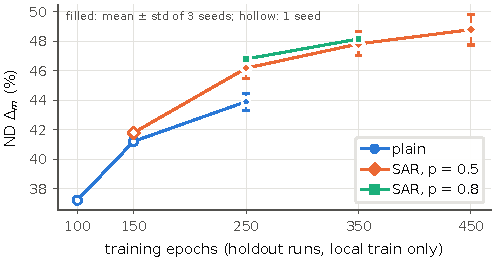
\includegraphics[width=\linewidth]{figs/epochs_fuse_b1_jd0.5.pdf}
  \vspace{-5.5mm}
  \caption{\textbf{ND $\Delta_m$ against epochs} (holdout runs): SAR augmentation keeps its lead as training gets
  longer.}
  \label{fig:epochs}
\end{figure}

\begin{figure}[t]
  \centering
  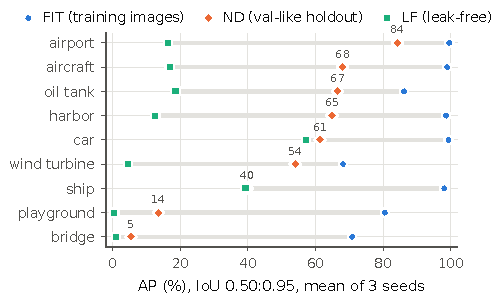
\includegraphics[width=\linewidth]{figs/per_class.pdf}
  \vspace{-5.5mm}
  \caption{\textbf{Per-class AP of the final recipe} on training images (FIT), the val-like holdout (ND) and leak-free
  scenes (LF), 3 seeds.}
  \label{fig:perclass}
\end{figure}

\begin{figure*}[t]
  \centering
  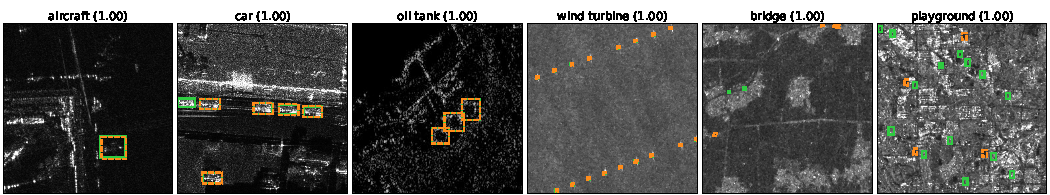
\includegraphics[width=\linewidth]{figs/qualitative.pdf}
  \vspace{-5.5mm}
  \caption{\textbf{Random ND images} (seed 0, one per class; not hand-picked) predicted by a holdout-trained model of
  the final recipe. Green: ground truth; orange: predictions with score $\ge$ 0.25. All are classified correctly; the
  objects of the first four classes are found, most bridges and playgrounds are missed.}
  \label{fig:qualitative}
\end{figure*}

\paragraph{Fitting versus generalising.}
\Cref{fig:perclass} splits the final recipe's ND mAP of 50.9: the model fits training scenes almost perfectly (FIT
89.0) but reaches 18.6 on leak-free ones.
Classes whose ND images mostly have partners (airport, oil tank, harbor, wind turbine: 83--100\,\%) inherit their fit;
car and ship generalise (LF 57 and 39); bridge and playground fail on both (ND 5 and 14).
Their boxes are as small as wind turbines', but they sit in cluttered scenes where similar structures carry no box,
and only 13\,\% and 36\,\% of their ND images have a partner: they are missed, not mislocated (\cref{fig:qualitative}).
Neither a stride-4 level (ND bridge AP 4.5 $\to$ 4.9) nor pasting their boxes into other images (val within seed noise)
fixed this; it is where our remaining gap lies.

\paragraph{From holdout to leaderboard.}
Holdout gains kept their sign on val but shrank: decoding +0.61 $\to$ +0.28, SWA +0.22 $\to$ +0.14.
Training on all of train instead of local train is worth about 10 $\Delta_m$ on val, as the extra images include
partners of val scenes.
Seven seeds of the final recipe span val $\Delta_m$ +43.8 to +45.9 (mean +44.9\,$\pm$\,0.7), a spread larger than most
single effects: hence our 3-seed rule, and the caveat that the posted seed is the best of eight on val.
\Cref{fig:epochs} shows why longer training paid off: ND kept rising with fit while LF stayed near 16--18 mAP.
Overfitting appears only far beyond our schedule: at batch 96, 700 and 1{,}000 epochs lowered val from +44.6 to
+42.9 and +41.7.
